\subsection{Setup}
We evaluate the performance of the proposed method across two datasets: a mathematical reasoning dataset (GSM8K, \citet{cobbe2021training}) and a logical reasoning dataset (ARC-Challenge, \citet{DBLP:conf/naacl/TalmorHLB19}). The sizes of the datasets are listed in \Cref{tab:datasets}.

\begin{wraptable}{r}{0.47\textwidth}
    \caption{Size of the Datasets}
    \vspace{-1em}
    \label{tab:datasets}
    \begin{center}        
    \def\arraystretch{1}
    \begin{tabular}{c|cc}
        \toprule
        \bf Name & \bf Training & \bf Evaluation \\
        \hline
        GSM8K & 7473 & 1319 \\
        ARC-Challenge & 1119 & 1172 \\
        \bottomrule
    \end{tabular}
    \vspace{-1em}
    \end{center}
\end{wraptable}

\paragraph{Training.}
For each dataset, we fine-tune three base models: Phi-3.5-mini-instruct~\citep{DBLP:journals/corr/abs-2404-14219}, Mistral-7B-Instruct-v0.3~\citep{DBLP:journals/corr/abs-2310-06825}, and Meta-Llama-3.1-8B-Instruct~\citep{DBLP:journals/corr/abs-2407-21783}, abbreviated as Phi-3.5, Mistral-7B, and Llama-3.1-8B, respectively. We provide two baseline comparisons: the base model and the supervised fine-tuned (SFT) model. For GSM8K, LaTRO fine-tuning excludes golden rationales from the solutions in the training set, while the SFT model is trained using golden rationales. For ARC-Challenge, as suggested in~\citep{zheng2024large}, the model is trained to generate answers to the text of multiple-choice questions rather than selecting labels. Since no golden rationales are available for ARC-Challenge, the SFT model is trained to directly generate answers.

\paragraph{Evaluation.}
For GSM8K, we evaluate all models with CoT prompting, and for ARC-Challenge, we evaluate the SFT baseline with direct answer generation, while the base model and the LaTRO fine-tuned model with CoT prompting. All evaluations are conducted with zero-shot prompts. We report both greedy decoding (GD) results and self-consistency (with temperature $T=1$) results. We choose a self-consistency sample size $k=8$ (maj@8) in \Cref{tab:main_experiment} after observing that more than 8 samples did not bring further performance improvement (see \Cref{fig:ablation}~(b) for details).

\paragraph{Implementation.} LaTRO is implemented on the high level as in \Cref{alg:latro_pseudocode}, with additional engineering techniques as discussed in \cref{sec:sampling_control}. LaTRO is implemented using the widely recognized transformers \citep{wolf-etal-2020-transformers} and TRL \citep{vonwerra2022trl} libraries, with PyTorch \citep{Ansel2024PyTorch2F} as backend. DeepSpeed ZeRO \citep{DBLP:conf/kdd/RasleyRRH20} is used in stage 3, along with Flash Attention 2 \citep{DBLP:conf/nips/DaoFERR22} to enhance training efficiency. The models were trained on a machine 
 equipped with 8xH100 80GB GPUs, using bfloat16 precision. %Hyperparameter selections are detailed as follows.
\paragraph{Hyperparameters.} AdamW optimizer with a learning rate of $5\times 10^{-7}$, no warm-up steps, and a linear decay strategy is used. The Monte Carlo (MC) sample size $K=16$ and the batch size of the data loader $3$ are predetermined, resulting in an effective batch size of $48$. Gradient accumulation steps and training batch size are subsequently adjusted to prevent out-of-memory errors during training.
A temperature of $T=1$ is used for MC sampling, and a penalty factor $\gamma=2$ is applied for incomplete rationales. The KL penalty is set at $\beta=0.05$ for GSM8K and $0.25$ for ARC-Challenge. Except for the results presented in \Cref{sec:ablation}, the maximum generation length is maintained at $L=500$. We train all models up to six epochs for GSM8K, and 12 epochs for ARC-Challenge. The checkpoint with best test accuracy is chosen.

For the SFT baseline experiments, we use a batch size of $32$ and adjust the learning rate to ensure that the evaluation loss decreases and finally converges. All SFT baselines are trained for a maximum of 12 epochs. The checkpoint with the best test accuracy is selected. 

In addition to the main quantitative results, we conduct ablation studies on two factors: 1. The maximum generation length $L$, where we study the effects of tuning $L$ in both training and inference times; 2. The self-consistency samples $k$, where we explore to what extent LaTRO can still benefit from inference-time scaling.

The main quantitative results, qualitative analysis of sample responses, and results of the ablation study are presented in \Cref{sec:results,sec:analysis,,sec:ablation}, respectively. Additional details on our prompt templates and more samples can be found in \Cref{sec:templates,sec:sample}.

\subsection{Results}
\label{sec:results}

In this subsection, we present evaluation results that demonstrate how effectively LaTRO enhances the reasoning abilities of LLMs on downstream datasets. The detailed results are provided in\Cref{tab:main_experiment}.

For the GSM8K dataset, LaTRO fine-tuned models outperform all base models by up to $19.5\%$ (Mistral-7B, $47.8\%\rightarrow 67.3\%$) and show an average improvement of $12.5\%$ across the three models examined with greedy decoding. The greatest improvement margin is observed for Mistral-7B, while the smallest is seen for Llama-3.1-8B, consistent with our initial findings in \Cref{fig:logprob_comparison}, where Mistral-7B exhibited the lowest log probability for directly answering questions and Llama-3.1-8B exhibited the highest. With self-consistency, the improvements are by up to $16.5\%$ (Phi-3.5, $74.0\% \rightarrow 90.5\%$) and the average improvement is $13.1\%$. Furthermore, LaTRO models demonstrate superior performance relative to SFT baselines, with an average improvement of $9.6\%$ for greedy decoding and $13.2\%$ for self-consistency. It is worth noting that for the SFT baseline of Llama-3.1-8B, overfitting on the test set is still observed after tuning the learning rate.

For ARC-Challenge, LaTRO fine-tuned models still outperform the baselines, though with a smaller margin. When using greedy decoding, the improvements over the base models are up to $1.6\%$ with an average increase of $1\%$. We see more increment with self-consistency, where the improvement margins are on average $2.4\%$. Comparing to SFT baslines, we find that all three models are very sensitive when fine-tuning to directly generate the answer of ARC-Challenge questions. They perform even inferior to the unoptimized base models. When using greedy decoding, the improvements of LaTRO fine-tuned models over the SFT baselines are on an average of $5.2\%$, and by up to $6\%$ (Llama-3.1-8B). In the case of self-consistency, LaTRO performs better than the base models by an average of $2.4\%$, and surpasses the SFT models by an average of $8.1\%$.
On the less surprising results compared to GSM8K, we conjecture that for ARC-Challenge, the models are already good at producing the answer either directly or through CoT prompting. Hence, further optimization of the reasoning process did not yield significant improvement.

% \haolincomment{Decide later if to add: This also aligns with the findings in \citet{sprague2024cot}, where the authors claimed that CoT only substantially helps with problems that require mathematical, logical, or algorithmic reasoning.}

% \zuxin{We'd better highlight the analysis in the Table, because people may not read the analysis carefully but just look at the results and wonder why we perform poorly on CommonsenseQA. For example, mark GSM8K and ARC as a category that require extensive reasoning and CommonsenseQA as another type.}

% \haolincomment{csqa may be a too easy task for complex reasoning, cite TO COT OR NOT TO COT?CHAIN-OF-THOUGHT HELPS MAINLY ON MATH AND SYMBOLIC REASONING}
% \haolincomment{Here all evaluations are done with $L=500$}

\begin{table}[t]
    \caption{Zero-shot accuracy (\%) comparison between LaTRO and the baselines on GSM8K and ARC-Challenge datasets. The models are fine-tuned on corresponding training datasets. The base model are marked with ``N/A'' in the training method. GD stands for greedy decoding at inference time and maj@8 stands for self-consistency with 8 samples. The models are evaluated by default using CoT, except that $\dagger$ indicates the direct answer generation is applied during evaluation. }
    \label{tab:main_experiment}
    \begin{center}
    %\renewcommand{\arraystretch}{1.35}
    \def\arraystretch{1.3}
    \begin{tabular}{lllcc}
        \toprule
        \bf Base Model & \bf Training Method & \bf Inference Method & \bf GSM8K  & \bf ARC-Challenge \\ 
        \hline
        \multirow{6}{*}{Phi-3.5} & \multirow{2}{*}{N/A} & GD & 72.9 & 85.1 \\
        & & maj@8 & 74.0 & 86.0 \\
        & \multirow{2}{*}{SFT} & GD & 75.8 & 81.0\textsuperscript{$\dagger$} \\
        & & maj@8 & 77.1 & 80.5\textsuperscript{$\dagger$} \\
        & \multirow{2}{*}{LaTRO} & GD & \bf 87.6 & \bf 86.4 \\
        & & maj@8 & \bf 90.5 & \bf 87.5\\
        \hline
        \multirow{6}{*}{Mistral-7B} & \multirow{2}{*}{N/A} & GD & 47.8 & 74.1 \\
        & & maj@8 & 58.2 & 74.1 \\
        & \multirow{2}{*}{SFT} & GD & 57.2 & 70.0\textsuperscript{$\dagger$} \\
        & & maj@8 & 59.9 & 70.6\textsuperscript{$\dagger$} \\
        & \multirow{2}{*}{LaTRO} & GD& \bf 67.3 & \bf 74.3 \\
        & & maj@8 & \bf 73.8 & \bf 78.9 \\
        \hline
        \multirow{6}{*}{Llama-3.1-8B} & N/A & GD & 76.8 & 81.4\\
        & & maj@8 & 79.7 & 84.4 \\
        &  \multirow{2}{*}{SFT} & GD & 73.2 & 77.0\textsuperscript{$\dagger$} \\
        & & maj@8 & 74.7 & 76.4\textsuperscript{$\dagger$} \\
        & \multirow{2}{*}{LaTRO} & GD& \bf 80.1 & \bf 83.0 \\
        & & maj@8 & \bf 87.0 & \bf 85.3\\
        \bottomrule
    \end{tabular}
    \end{center}
    
\end{table}


\begin{figure}[t]
    \centering
     \begin{tabular}{cc}
     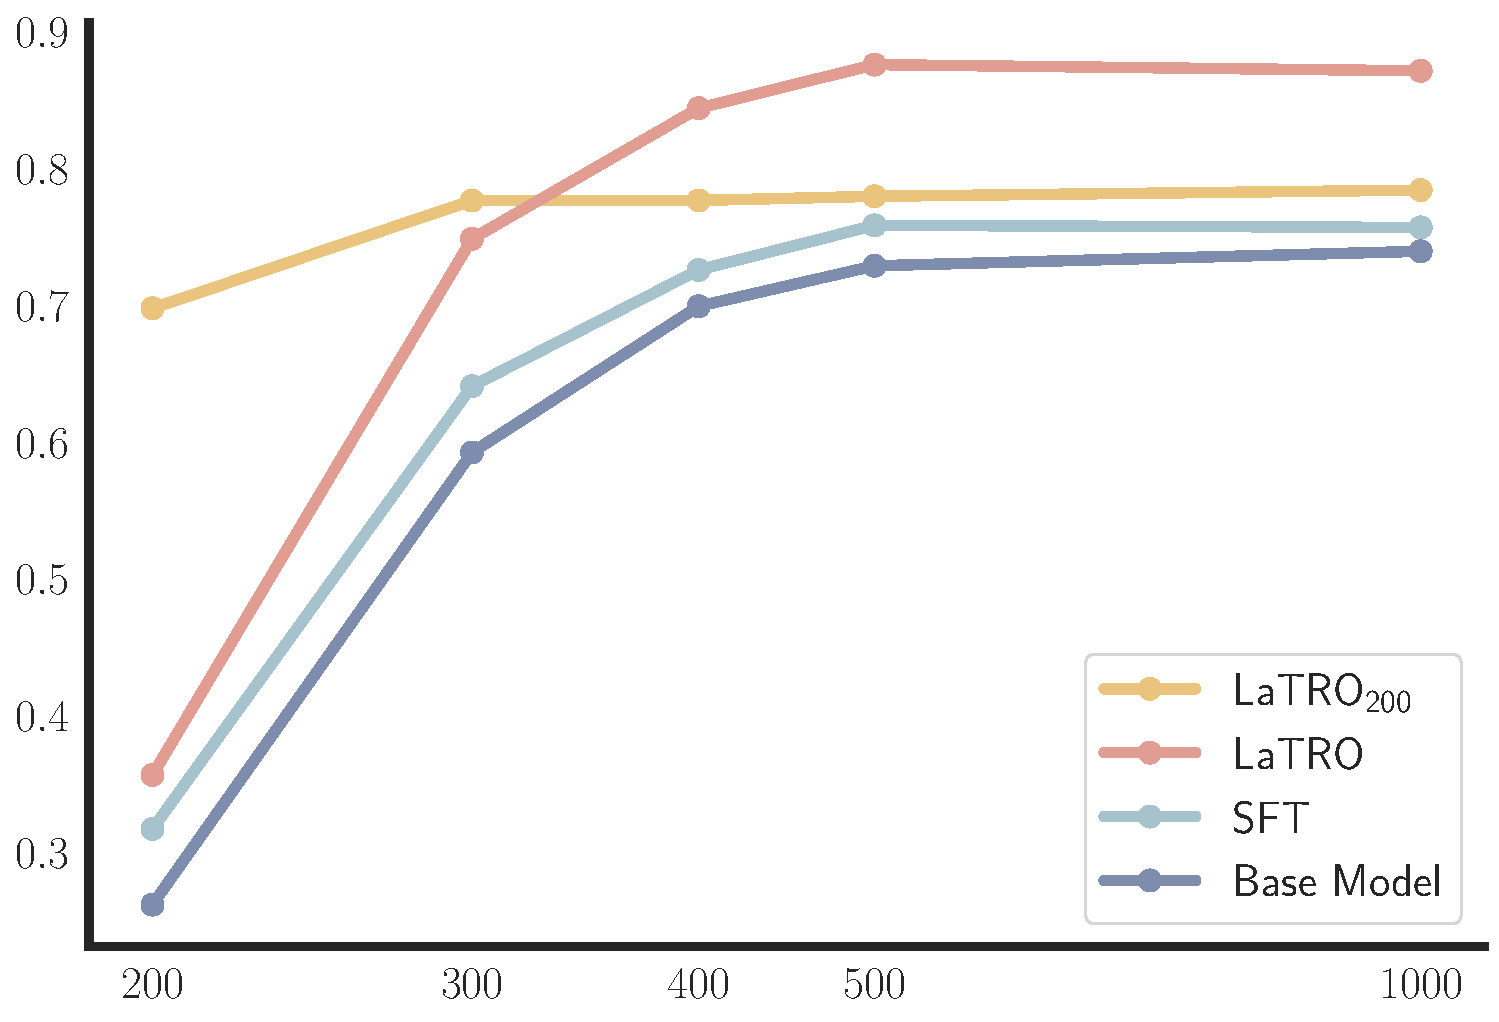
\includegraphics[width=.47\linewidth]{figures/ablation_study_token_length.pdf} &
     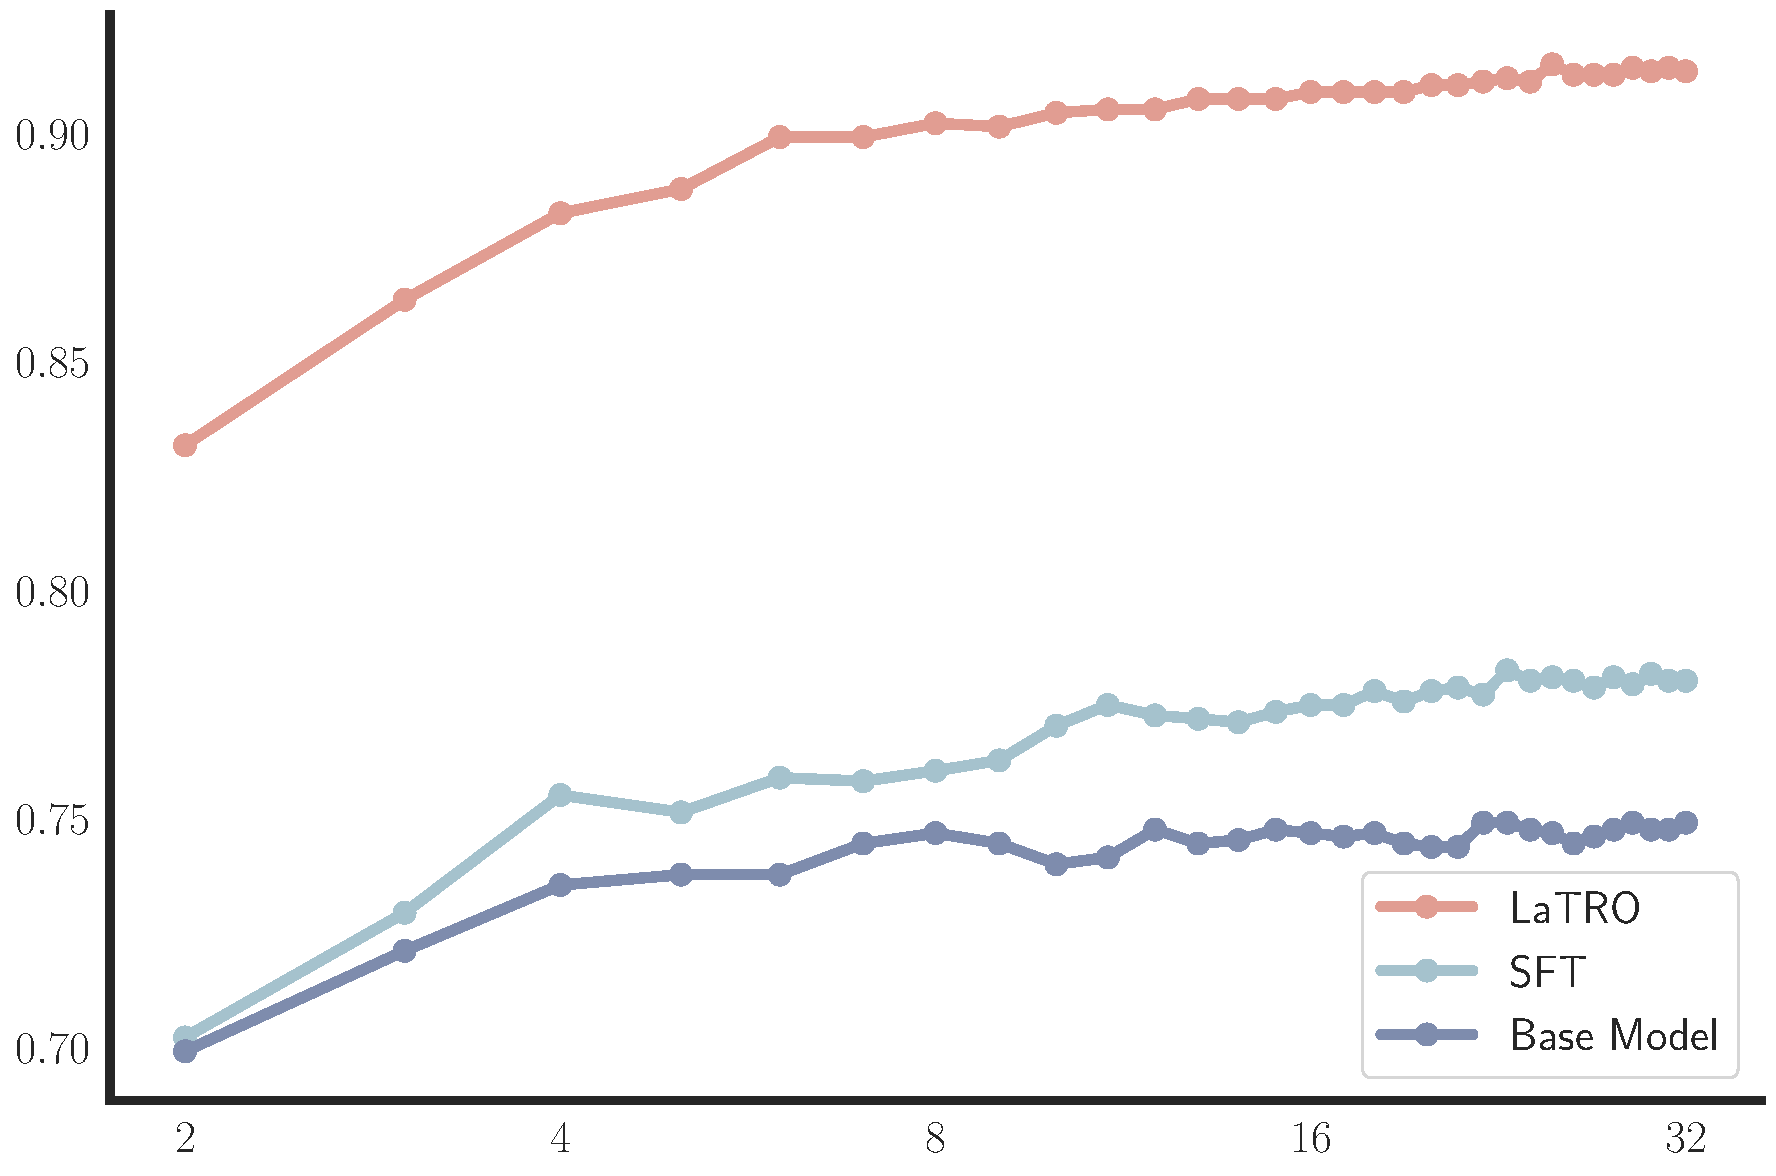
\includegraphics[width=.47\linewidth]{figures/self_consistency.pdf} \\
     \small{(a) Zero-shot accuracy with different $L$.} & \small{(b) Zero-shot maj@$k$ accuracy with different $k$.}
     \end{tabular}
    \caption{Ablation study results on GSM8K with base model Phi-3.5. In (a), the $x$-axis represents various maximum token length $L$ of reasoning rationales, $y$-axis is the accuracy, and the plot shows the zero-shot performance v.s. various maximum token lengths for different methods. In (b), the $x$-axis represents the \# of sampled reasoning rationales, the $y$-axis is the accuracy, and the plot shows the zero-shot performance v.s. the  \# of reasoning rationales used in the majority vote.}
    \label{fig:ablation}
\end{figure}



\subsection{Ablation Study}
\label{sec:ablation}

In this subsection, we present our ablation study on the effect of different parameters in LaTRO. For consistency, we fix the base model to Phi-3.5 and the dataset to GSM8K throughout the ablation experiments.

% \subsubsection{How many tokens are enough?}
\paragraph{How many tokens are enough?} \citet{DBLP:conf/iclr/0001LZ024} demonstrated that when the input length is $n$, a transformer model with a hidden size of $O(\log n)$ can solve problems equivalent to Boolean circuits of size $m$, using $m$ CoT steps. However, the empirical determination of sufficient CoT tokens for optimal performance remains underexplored. In this section, we report zero-shot accuracy with generation length $L$ ranging from 200 to 1000 tokens at inference time. Additionally, a Phi-3.5 model is fine-tuned with $L=200$ for comparison. We distinguish two LaTRO fine-tuned models, referred to as LaTRO and $\text{LaTRO}_{200}$. As shown in~\Cref{fig:ablation}(a) accuracy gains plateau when $L\geq 500$, suggesting 500 tokens might suffice for grade school math problems. In contrast, limiting $L$ to 200 reduces accuracy, unless the model is trained accordingly. Interestingly, LaTRO significantly improves performance under this constraint by training the model to generate more concise rationales. This finding implies LaTRO can also train LLMs to condense rationales for limited inference-time compute. A sample from $\text{LaTRO}_{200}$ is provided in \Cref{sec:sample} for qualitative analysis.


% \begin{figure}[t]
%     \centering
%     \begin{minipage}{0.45\textwidth}
%         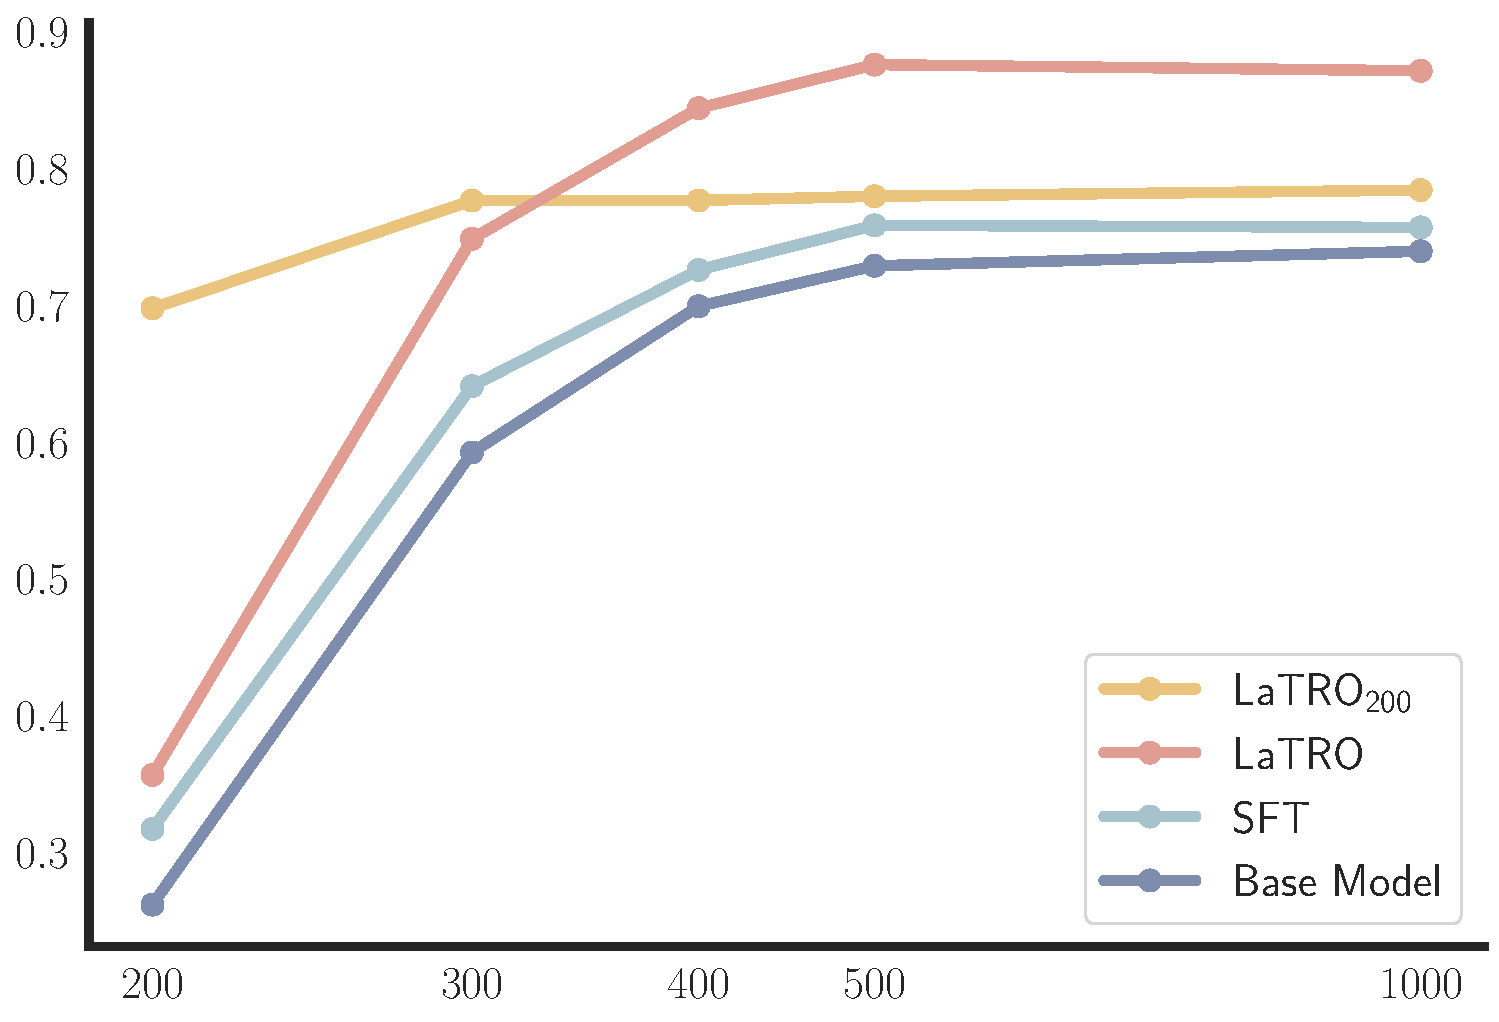
\includegraphics[width=\textwidth]{figures/ablation_study_token_length.pdf}
%         \caption{Zero-shot accuracy in GSM8K with different $L$}
%         \label{fig:token_length_vs_acc}
%     \end{minipage}
%     \hfill
%     \begin{minipage}{0.45\textwidth}
%         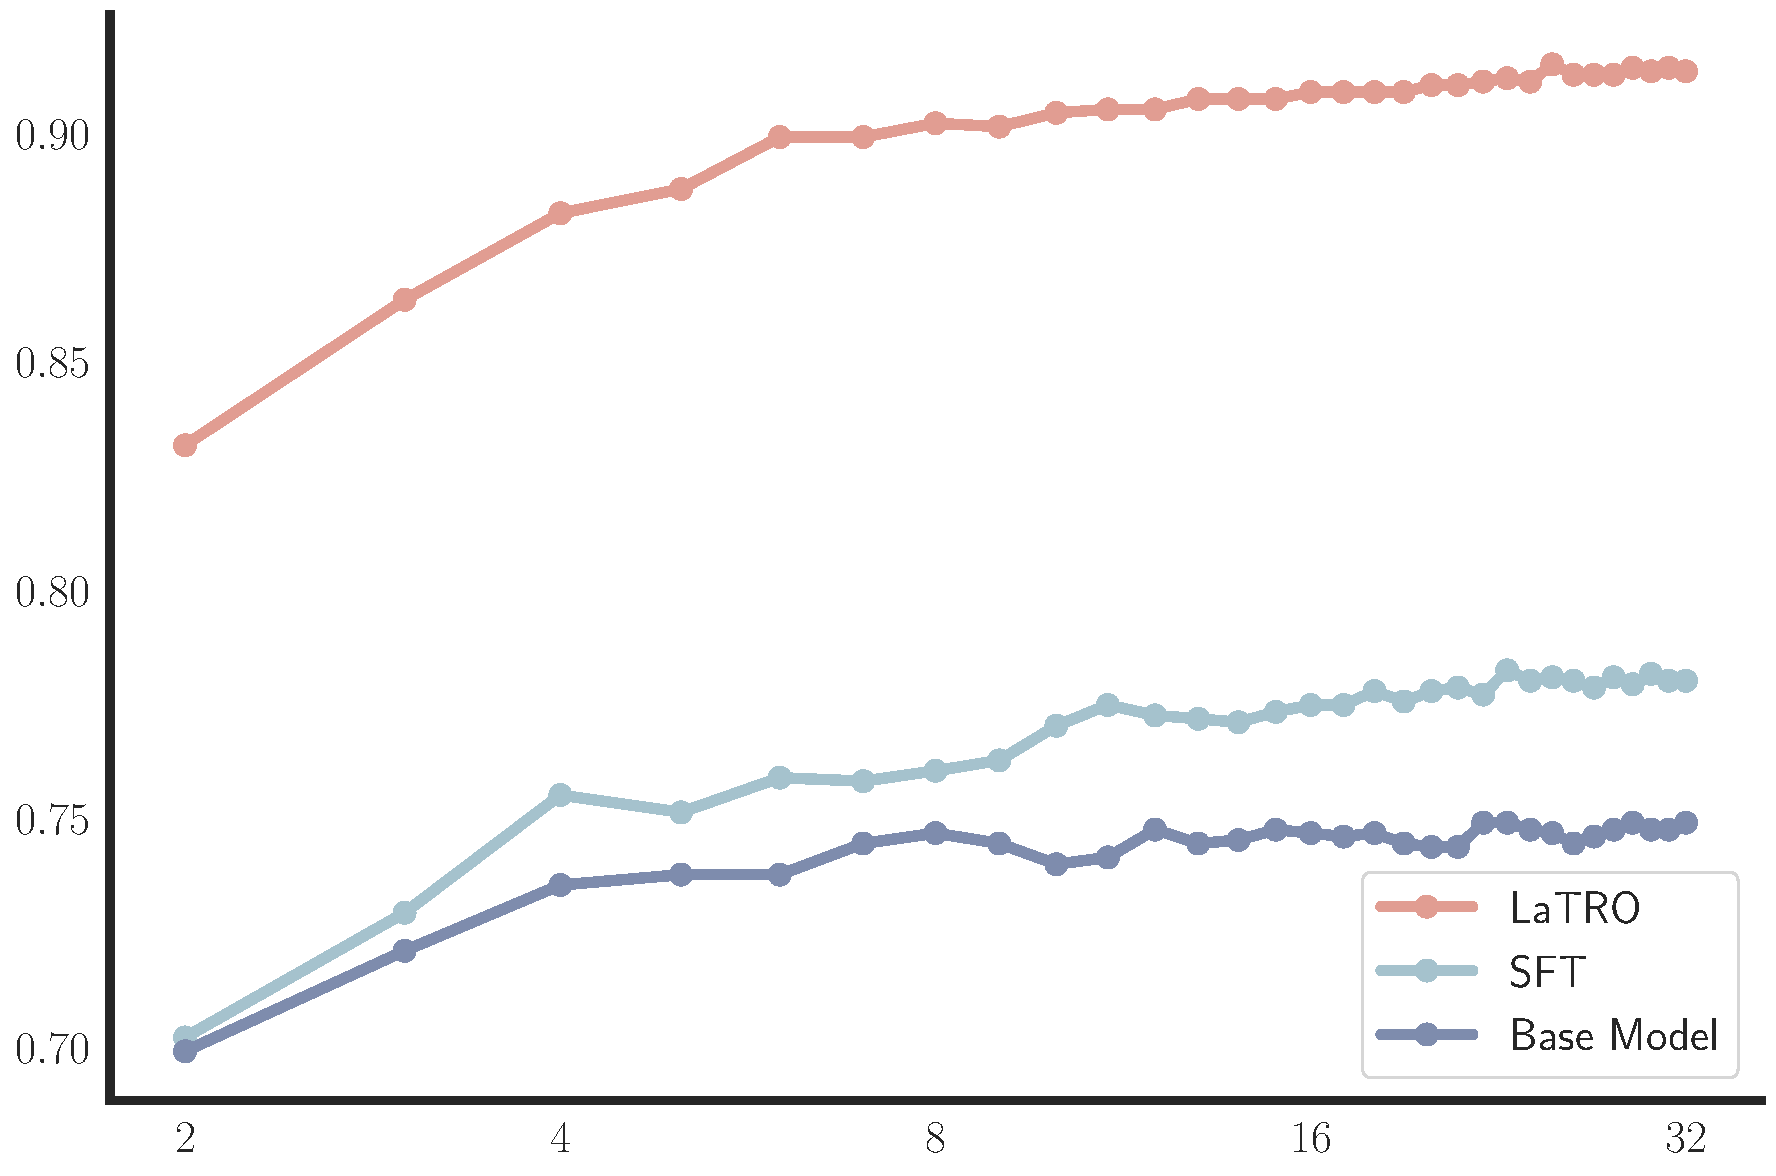
\includegraphics[width=\textwidth]{figures/self_consistency.pdf}
%         \caption{Zero-shot maj@$k$ accuracy in GSM8K with different $k$}
%         \label{fig:self_consistency}
%     \end{minipage}
% \end{figure}
%\subsubsection{How much inference-time scaling is enough?}

\paragraph{Is inference-time scaling still beneficial?} While LaTRO shifts much of the reasoning computation to training time, it can still benefit from the inference-time scaling. To explore this, We evaluate the models again using self-consistency with the number of samples $k$ ranging from 1 to 32. As shown in~\Cref{fig:ablation} (b), with $k=8$ rationales and majority voting, LaTRO achieves 90\% accuracy on GSM8K. This indicates that LaTRO equipped with self-consistency can further enhance performance, even with LaTRO's focus on training-time optimization.


\begin{figure}[ht]
    \centering
    \begin{bluetextbox}
        \setstretch{1.1}
        \textbf{Question}: Frankie and Binkie went bowling together. Frankie's score was 15 better more than twice as high as Binkie's. If Binkie bowled a score of 90, what was Frankie's score? Let's think step by step.

        \textbf{Response (Base model)}: Let's break this problem down into steps:
        
        1. We know that the difference between Frankie's score (F) and Binkie's score (B) is 15. So we can express Frankie's score as \textcolor{red}{F = B + 15}
        
        2. We also know that Frankie's score is twice as high as Binkie's score. So we can write another equation: F = 2B
        
        3. Now, we have two equations with two unknowns. Let's solve for Frankie's score (F) by setting the two equations equal to each other:
        - 2B = B + 15
        - Multiply both sides by 1 to get rid of the fraction: 2B - B = 15
        - Simplify: B = 15 (since subtracting B from 2B results in 15)
        
        4. Now that we know Binkie's score, we can find Frankie's score using either of the equations we created earlier. Let's use the first one (F = B + 15):
        - F = 15 + 15
        - Frankie's score is 30 more than Binkie's score, which is 15 in this case. So Frankie's score is 15 + 15 = 30 + 15 = 45
        
        The final answer is that Frankie's score was 45.

        \textbf{Reponse (SFT)}: Twice as many as Binkie's 90 score is equal to 2*90= <<2*90=180>>180. Therefore, \textcolor{red}{180-(180-15)=165} was the number Frankie bowled. The answer is 165

        \textbf{Response (LaTRO)}: Here's how to solve the problem:
        1. We know that Binkie's score is 90.
        2. The problem states that Frankie's score was 15 better more than twice as high as Binkie's score. This means that Frankie's score is 15 + (2 * 90) = 15 + 180 = 195.

    \end{bluetextbox}
    % \begin{bluetextbox}
    %     \textbf{Question}: Jeff’s work is 3 miles away.  He walks there and back each day he works.  How many miles does he walk if he has to work 5 times a week? Let's think step by step.
    
    %     \textbf{Response (Base model)}: First, let's find out how many miles Jeff walks each day when he works: 1. He walks 3 miles to his work and 3 miles back, so he walks 6 miles for one day.
    
    %     Next, let's find out how many miles he walks in a week if he works 5 days:
    
    %     1. He walks 6 miles each day, so he walks 6 miles * 5 days = 30 miles in a week.
    
    %     So, Jeff walks 30 miles if he has to work 5 times a week.
    
    
    %     \textbf{Response (SFT)}: Each day of work he walks 2 miles because 3 miles/day + 3 miles/day = <<3+3=6>>6 miles. But he walks 5 days a week, so he walks a total of 30 miles a week because 5 days X 2 miles/day = <<5*2=10>>10 miles. The answer is 10.
    
    
    %     \textbf{Response (LaTRO)}: Here is the solution to the problem:
        
    %     1. Jeff walks 3 miles each way he goes to work, so he walks 3 + 3 = 6 miles each day he works.
        
    %     2. If he works 5 times a week, he will walk 6 * 5 = 30 miles each week.
    
    % \end{bluetextbox}
    \caption{Sample responses of a GSM8K question from Mistral-7B models, the errors are highlighted in red.}
    \label{fig:samples_mistral}
\end{figure}



\subsection{Case study}
\label{sec:analysis}
 We take a closer look at the responses generated by the LaTRO fine-tuned models. 
 We select a question from GSM8K and compare the responses from the base, the SFT model, and the LaTRO finetuned model. 
 We choose the set of responses from the Mistral-7B models that we evaluated. As can be seen in \Cref{fig:samples_mistral}, the base model not only generates a lengthy response, it also makes a logical mistake at the first step, where the correct equation to establish here is ``F = 2B + 15''. The SFT model simplifies the answer and makes the first step correct. However, in the second step it first makes a wrong equation, then makes an arithmetic error when evaluating this equation. Further, LaTRO can give a concise and correct answer. We include more sample responses in \Cref{sec:sample}.
